\documentclass[11pt]{article}
\usepackage[margin=1in]{geometry}
\usepackage{amsmath,amssymb,amsfonts}
\usepackage{graphicx, float}
\usepackage{fancyhdr,booktabs}
\usepackage{listings}
\lstset{
    language=Python,
    basicstyle=\ttfamily\small,
    breaklines=true,
    keepspaces=true,
    showstringspaces=false
}

% Header and Footer Setup
\pagestyle{fancy}
\fancyhf{}
\lhead{Ph429 NLD \& Chaos -- Fall 2026}
\rhead{Problem Set 1}
\cfoot{\thepage}

\title{\textbf{Ph429: Nonlinear Dynamics \& Chaos}\\[0.5ex]\Large Problem Set 1}
\author{Zeshui Song}
\date{Fall 2026}

\begin{document}
\maketitle

\vspace{-1em}

\subsection*{Problem 0}
Look up the logistic differential equation and its sigmoid growth curve in a calculus book. The goal is to understand:
\begin{enumerate}
    \item[(a)] how the logistic differential equation is solved, and
    \item[(b)] how what it describes is different from the iterative logistic model.
\end{enumerate}

\paragraph{Solution} 
The logistic differential equation is given by
\[\frac{dP}{dt}=rP\left(1-\frac{P}{K}\right)\]
Where:
\begin{itemize}
    \item $P$ is the population size at time $t$
    \item $r$ is the intrinsic growth rate of the population
    \item $K$ is the carrying capacity of the environment
\end{itemize}
It is solved through the method of separation of variables:
\[\frac{dP}{dt}=\frac{rP(K-P)}{K}\]
\[\frac{K}{P(K-P)}\,dP = r\,dt\]
Integrating both sides:
\[\int \frac{K}{P(K-P)}\,dP = \int r\,dt\]
Partial fraction decomposition of the left-hand side gives:
\[\frac{K}{P(K-P)} = \frac{1}{P} + \frac{1}{K-P}\]
\[\implies \int \left( \frac{1}{P} + \frac{1}{K-P} \right)\,dP = \int r\,dt\]
\[\implies \ln|P| - \ln|K-P| = rt + C\]
\[\implies \ln\left|\frac{P}{K-P}\right| = rt + C\]
\[\implies \frac{P}{K-P} = Ae^{rt}\]
where $A = e^C$ is a constant of integration. Solving for $P$ gives:
\[
P(t) = \frac{AK e^{rt}}{1 + A e^{rt}}
\]
Plug in the initial condition $P(t=0) = P_0$ to determine the constant $A$:
\[A=\frac{P_0}{K-P_0}\]
This results in the continuous sigmoid growth curve $P(t)$ shown below:
\begin{center}
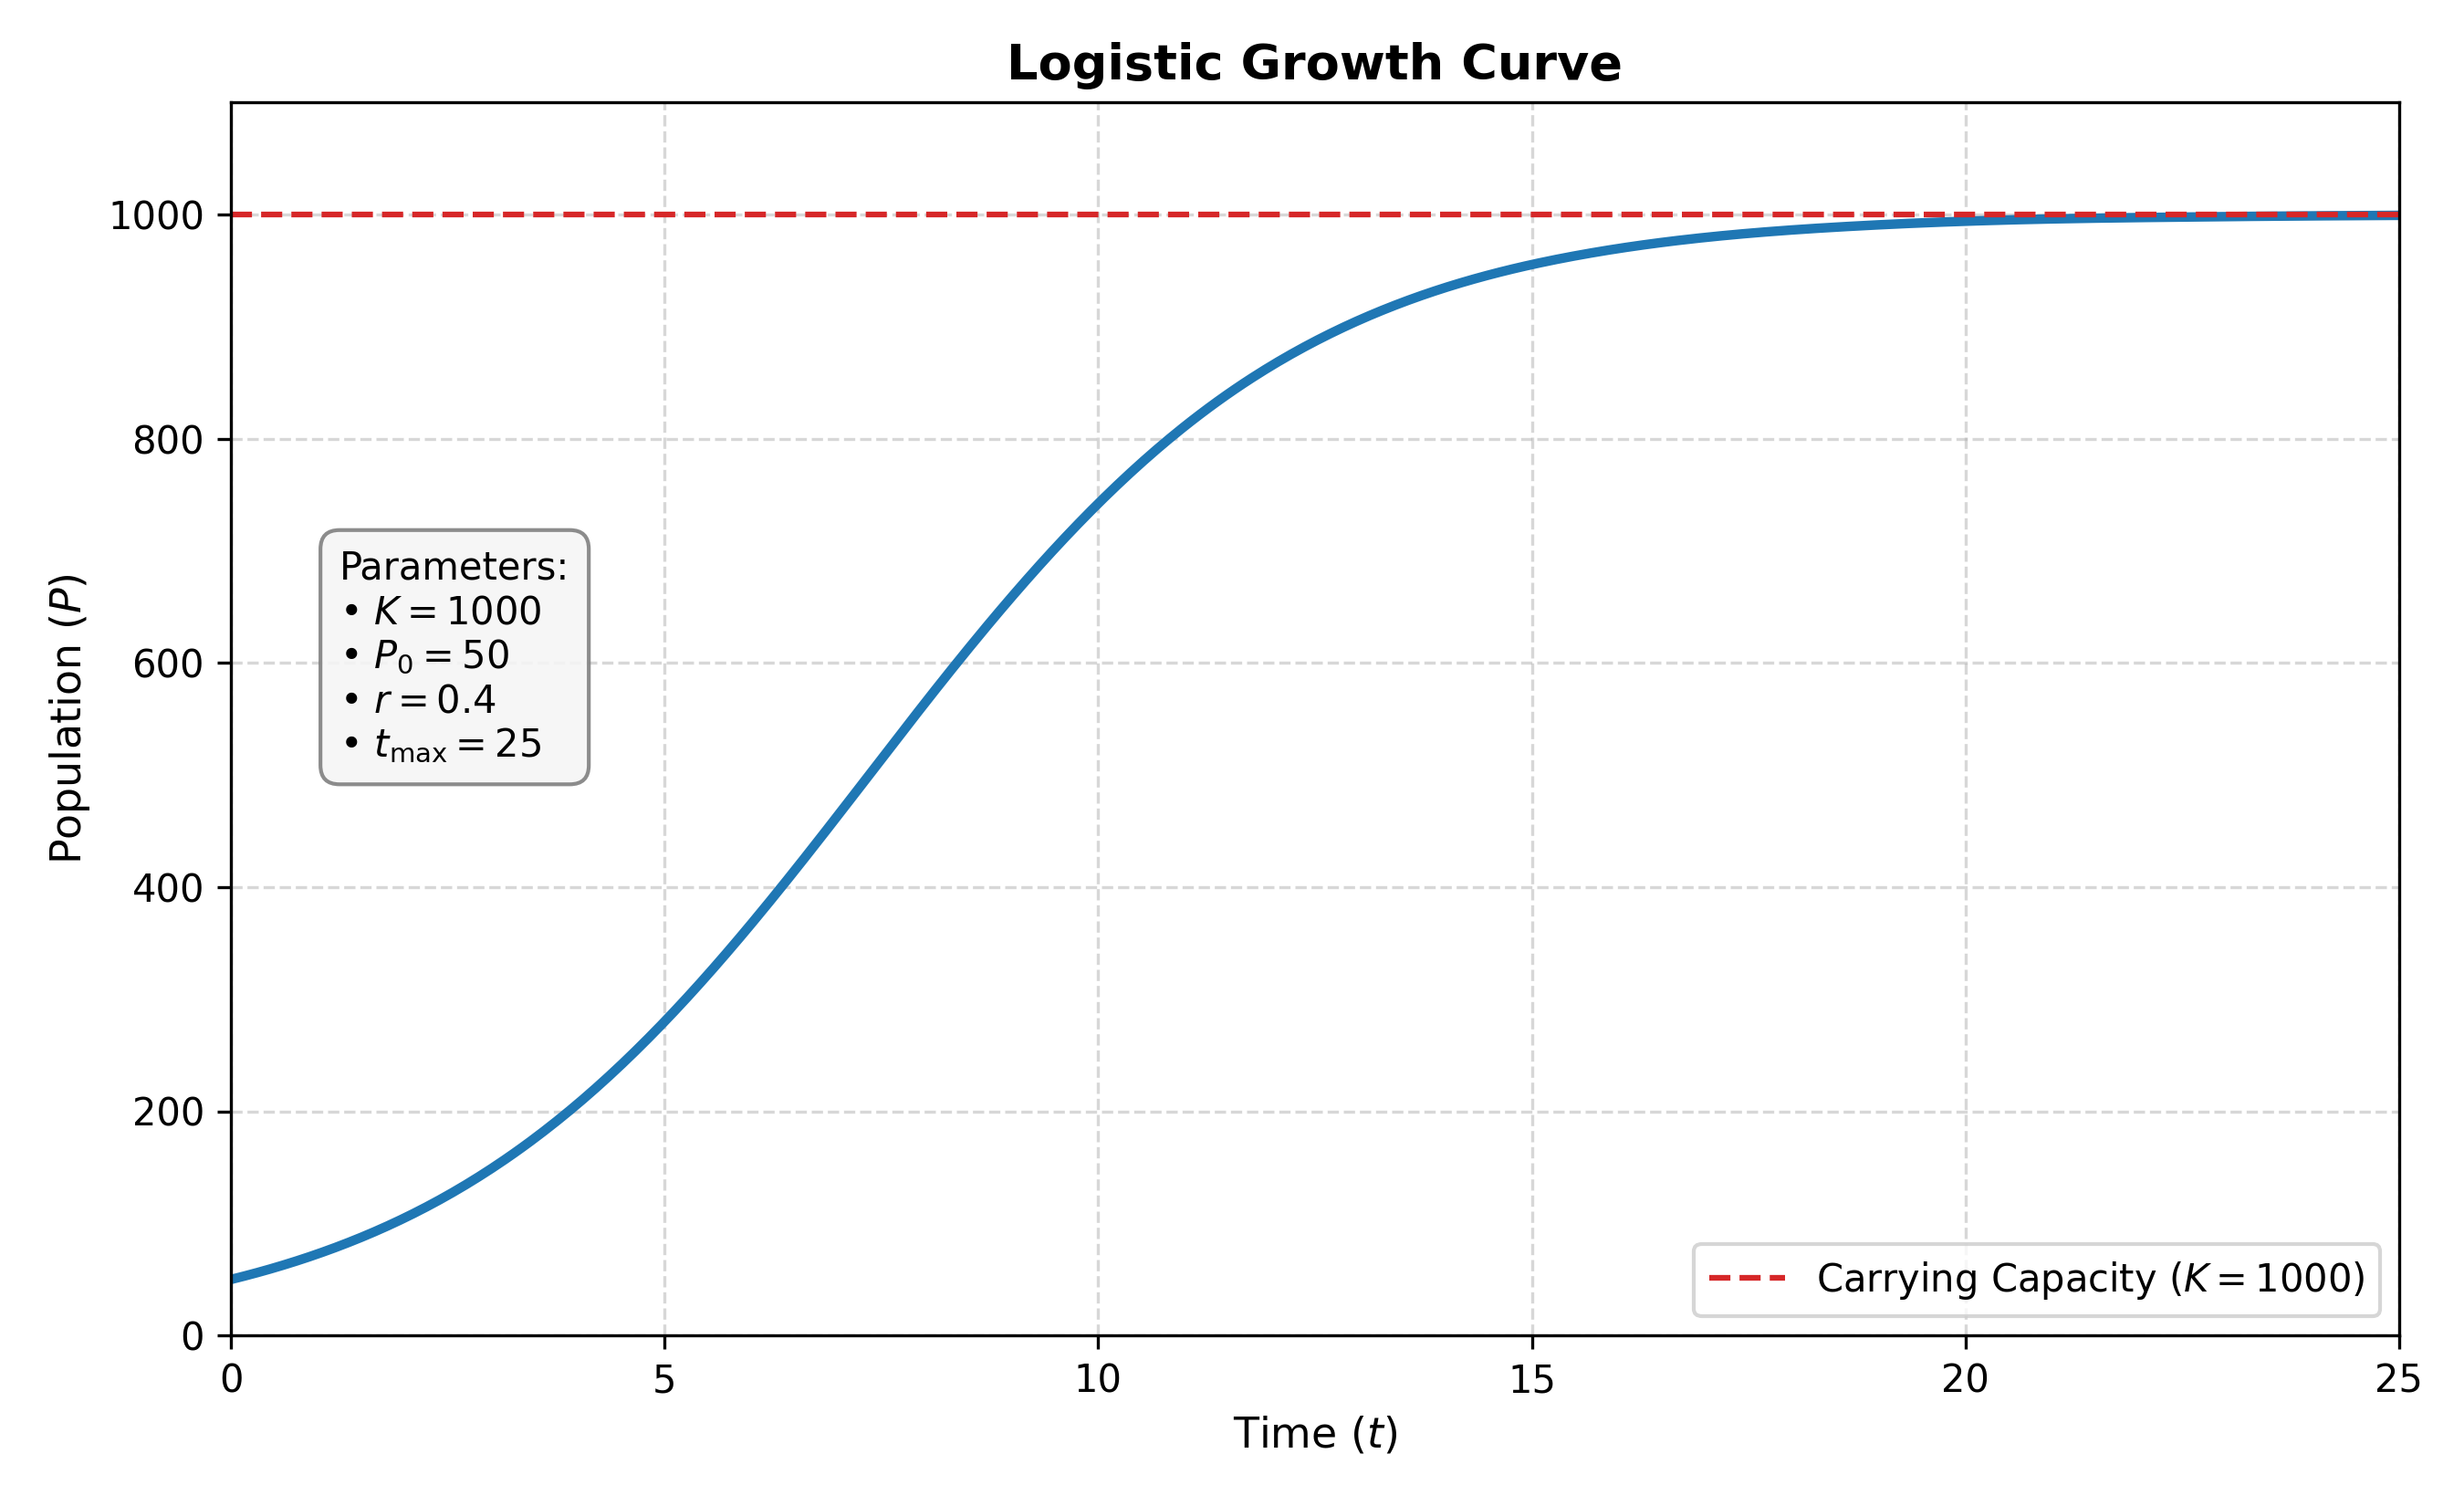
\includegraphics[width=0.8\textwidth]{Logistic DE.png}
\end{center}
\underline{Comparison to Iterative Logistic Model}\\
The solution to the logistic differential equation gives the continuous sigmoid growth curve for the population $P(t)$ over time $t$. However, the iterative logistic model $x_{n+1}=rx_n (1-x_n)$ describes a dynamics of a model in discrete time steps. Unlike the differential equation, the iterative model results in discontinuous outputs that jump between values, exhibiting varying behaviors such as periodic oscillations or chaos depending on the parameter $r$.

\newpage

\subsection*{Problem 1}
Study the map
\[
x_{n+1} = \sqrt{x_n}
\]
Iterate the map graphically or computationally. Find all fixed points and test their stability. Describe the behavior of the iterates for appropriate choices of the initial condition $x_0$.

\paragraph{Solution} Computationally, the map is iterated for various initial conditions $x_0$ until it converges to the fixed point $x^* = 1$ within a tolerance of $10^{-5}$.
\begin{table}[H]
  \centering
  \caption{Computational Iteration to Numerical Convergence}
  \begin{tabular}{c c l c}
    \toprule
    $x_0$ & Steps to Converge & First Six Iterates $(x_0, x_1, \dots, x_5)$ & Converged Value \\
    \midrule
    $0.1$ & 18 & $[0.1000,\, 0.3162,\, 0.5623,\, 0.7499,\, 0.8660,\, 0.9306]$ & $0.99999$ \\
    $0.5$ & 17 & $[0.5000,\, 0.7071,\, 0.8409,\, 0.9170,\, 0.9576,\, 0.9786]$ & $0.99999$ \\
    $3.5$ & 17 & $[3.5000,\, 1.8708,\, 1.3678,\, 1.1695,\, 1.0814,\, 1.0399]$ & $1.00001$ \\
    \bottomrule
  \end{tabular}
\end{table}
\begin{center}
    \includegraphics[width=\textwidth]{P1 time series.png}
\end{center}
\begin{center}
    \includegraphics[width=\textwidth]{P1 map.png}
\end{center}
\underline{Finding Fixed Points and their Stability}\\
In 10.1 of Strogatz, a fixed point $x^*$ of a map $x_{n+1} = f(x_n)$ is a value such that $f(x^*) = x^*$. The stability of the fixed point is determined using the linearized map $\eta_{n+1} = f'(x^*) \eta_n$ which describes the evolution of small perturbations $\eta_n$ around the fixed point.\\\\
If $|f'(x^*)| < 1$, the fixed point is stable ($\eta_n \to 0$ as $n \to \infty$) and the orbit is attracted to $x^*$. If $|f'(x^*)| > 1$, the fixed point is unstable ($\eta_n$ grows) and the orbit is repelled from $x^*$. However, if $|f'(x^*)| = 1$, then we have a marginal case, and higher-order terms in the Taylor expansion of $f$ must be considered to determine stability.\\\\
Thus, applying the above to the map $x_{n+1} = \sqrt{x_n}$, we have the following fixed points:
\[x^* = \sqrt{x^*} \implies {x^*}^2 = x^* \implies x^*(x^* - 1) = 0\]
\[x^* = 0 \text{ or } x^* = 1\]
To determine the stability of these fixed points, we compute the derivative of the map $f(x) = \sqrt{x}$:
\[
f'(x) = \frac{1}{2\sqrt{x}}
\]
Evaluating at the fixed points:
\[
f'(0) = \lim_{x \to 0^+} \frac{1}{2\sqrt{x}} = \infty, \quad f'(1) = \frac{1}{2}
\]
At the fixed point $x^* = 0$, the derivative is undefined (approaches infinity), but based on the behavior of the cobweb diagram, it behaves like an unstable fixed point. At the other fixed point, since $|f'(1)| = 1/2 < 1$, the fixed point $x^* = 1$ is stable.


\subsection*{Problem 2}
Study the map (same as for Problem 1):
\[
x_{n+1} = \tan(x_n)
\]

\paragraph{Solution}
The fixed point of the map is given by looking at the points of intersection where $f(x*) = \tan(x^*) = x^*$. The fixed points for the domain $[0, \pi/2)$ are:
\[\tan(x^*) = x^*\implies x^* = 0\]
To determine the stability of this fixed point, we compute the derivative of the map $f(x) = \tan(x)$ at the fixed points:
\[f'(x) = \sec^2(x)\]
\[f'(0) = \sec^2(0) = 1\]
Thus, the fixed point $x^* = 0$ is the marginal case where the test is inconclusive. We will need to consider the higher-order terms that were neglected for the linearized map $\eta_{n+1} = f'(x^*) \eta_n$. 
\[\eta_{n+1}
= f'(x^*)\eta_n
+ \underbrace{
    \frac{f''(x^*)}{2!}\eta_n^2
    + \frac{f'''(x^*)}{3!}\eta_n^3
    + \cdots
}_{O(\eta_n^2)}\]
\[f''(x) = 2\sec^2(x)\tan(x) \implies f''(0) = 0\]
\[f'''(x) = 2[2\sec^2(x)\tan^2(x) + 2\sec^4(x)] \implies f'''(0) = 4\]
Since $f'''(0) > 0$, the fixed point $x^* = 0$ is unstable.\\\\
Since the map does not have a stable fixed point, the following time series and cobweb diagram is generated for the specified initial conditions stopping after 60 iterations instead of convergence to a fixed point.
\begin{center}
    \includegraphics[width=\textwidth]{P2 time series.png}
    \includegraphics[width=\textwidth]{P2 map.png}
\end{center}

\subsection*{Problem 3}
Try to determine the Feigenbaum constant numerically for the map
\[
x_{n+1} = a \sin(x_n)
\]
(find successive parameter values at which period-doubling occurs and use these to estimate the Feigenbaum constant).

\paragraph{Solution}
The graph of the sine map below shows a smooth, concave down curve with a single maximum at $x = \pi/2$ (for an arbitrary value of $a=2$). Thus, it is an unimodal map like the logistic map. According to 10.6 of Strogatz (universality), any unimodal map with exhibit the same convergence rate to chaos, and thus the expected Feigenbaum constant is $\delta \approx 4.669$.
\begin{center}
    \includegraphics[width=0.5\textwidth]{sine_map.png}
\end{center} 
\[\delta = \lim_{n\to\infty} \frac{a_n - a_{n-1}}{a_{n+1} - a_n}\approx 4.669\]
\underline{Approach}\\
I can estimate the Feigenbaum constant numerically by finding the parameter values $a_n$ at which the first three period-doublings occur based on example 10.3.3.
\begin{itemize}
    \item Period 1 (fixed point) to period 2:\\
    A fixed point $x^*$ is stable when the multiplier satisfies $|f'(x^*)| < 1 \implies -1 < f'(x^*) < 1$. The period-doubling occurs at the parameter boundary $a_1$ where stability is lost through the lower bound:
    $$f'(x^*) = -1 \quad \text{with } f(x^*) = x^*$$

    \item Period 2 to period 4:\\
    The 2-cycle $\{p, q\}$ consists of fixed points of the \textit{second iterate} $f^2(x) = f(f(x))$, which is stable when $|(f^2)'(p)| < 1 \implies -1 < (f^2)'(p) < 1$. The period-doubling occurs at the parameter boundary $a_2$ where stability is lost through the lower bound:
    $$(f^2)'(p) = \frac{d}{dx}\Big(f(f(x))\Big)\bigg|_{x=p} = f'(f(p))f'(p) = f'(q)f'(p) = -1$$
    $$\text{Where } f(p) = q \text{ and } f(q) = p \ (p \neq q)$$

    \item Period 4 to period 8:\\
    The 4-cycle $\{x_1, x_2, x_3, x_4\}$ consists of fixed points of the \textit{fourth iterate} $f^4(x) = f(f(f(f(x))))$, which is stable when $|(f^4)'(x_1)| < 1 \implies -1 < (f^4)'(x_1) < 1$. The period-doubling occurs at the parameter boundary $a_3$ where stability is lost through the lower bound:
    $$(f^4)'(x_1) = \prod_{k=1}^4 f'(x_k) = f'(x_4)f'(x_3)f'(x_2)f'(x_1) = -1$$
    $$\text{Where } x_2 = f(x_1), \; x_3 = f(x_2), \; x_4 = f(x_3), \; x_1 = f(x_4)$$
    \item Feigenbaum constant:
    \[\delta \approx \frac{a_2 - a_{1}}{a_{3} - a_2}\]
\end{itemize}
System of equations for $a_1$:
\begin{eqnarray*}
    f'(x^*) = a\cos(x^*)=-1 \implies a\cos(x^*) + 1&=0\\
    x^* = a\sin(x^*) \implies x^* - a\sin(x^*) &= 0
\end{eqnarray*}
System of equations for $a_2$:
\begin{eqnarray*}
    f'(p)f'(q) = a^2\cos(p)\cos(q)=-1 \implies a^2\cos(p)\cos(q) + 1 &=0\\
    q = a\sin(p)\implies q - a\sin(p) &= 0\\
    p = a\sin(q)\implies p - a\sin(q) &= 0
\end{eqnarray*}
System of equations for $a_3$:
\begin{eqnarray*}
    f'(x_1)f'(x_2)f'(x_3)f'(x_4) =-1 \implies a^4\cos(x_1)\cos(x_2)\cos(x_3)\cos(x_4) + 1 &=0\\
    x_2 = a\sin(x_1)\implies x_2 - a\sin(x_1) &= 0\\
    x_3 = a\sin(x_2)\implies x_3 - a\sin(x_2) &= 0\\
    x_4 = a\sin(x_3)\implies x_4 - a\sin(x_3) &= 0\\
    x_1 = a\sin(x_4)\implies x_1 - a\sin(x_4) &= 0
\end{eqnarray*}
Since the systems of equations are transcendental, I used the \texttt{fsolve} function in Python to numerically solve for the parameter values $a_1, a_2, a_3$ at which the first three period-doublings occur.\\\\
For example, the code below shows the solver for the period-doubling from period 2 to period 4. It works by first defining the system of equations and the unknown variables $p$ and $a$ (note that $q$ is not a separate unknown since it is defined in terms of $p$ and $a$). Then, starting guesses for the unknowns are found by iterating the map for a range of $a$ values and checking whether the cycle closure error is below $10^{-8}$ and the second equation ($a^2\cos(p)\cos(q)+1$) is between $0$ and $0.2$. Finally, the \texttt{fsolve} function is used with the starting guesses to find the solution for $p$ and $a_2$.
\begin{lstlisting}
# -------- Period 2 -> 4 --------

def equations2(values):
    p, a = values
    q = a * np.sin(p)

    return [
        a * np.sin(q) - p,
        a**2 * np.cos(p) * np.cos(q) + 1
    ]


# Find a starting guess automatically
for a in np.arange(1.1, 3.0, 0.01):

    p = 0.5
    for i in range(2000):
        p = a * np.sin(p)

    error, m = equations2([p, a])

    if abs(error) < 1e-8 and 0 < m < 0.2:
        break


# Solve and check
p, a2 = fsolve(equations2, [p, a])

error, m = equations2([p, a2])
valid2 = abs(error) < 1e-8 and abs(m) < 1e-8

if valid2:
    print("a2 =", a2)
else:
    print("Solver did not find a2")
\end{lstlisting}
\underline{Note:} The code for this solver was written using assistance from ChatGPT. The systems of equations were derived by me using the textbook examples and the code was written to numerically solve them.\\\\
Using a similar approach for the other two period-doublings, I found the following parameter values:
\begin{itemize}
    \item Period 1 to Period 2: $a_1 \approx 2.2618263341146543$
    \item Period 2 to Period 4: $a_2 \approx 2.6177834554109998$
    \item Period 4 to Period 8: $a_3 \approx 2.697399914889866$
\end{itemize}
Thus, the Feigenbaum constant is estimated as:
\[\delta = \frac{a_2 - a_1}{a_3 - a_2} \approx \boxed{4.47089}\]



\subsection*{Problem 4}
Assume $P_t$ represents the fraction of neurons of a large neural network that fire at time $t$. As a simple model of epilepsy, the dynamics of the network can be described by the finite-difference equation
\[
P_{t+1} = 4CP_t^3 - 6CP_t^2 + (1 + 2C)P_t,
\]
where $C$ is a positive parameter and $0 \le P_t \le 1$.

\begin{enumerate}
    \item[(a)] Find the fixed points.
    \item[(b)] Determine the stability at each fixed point and describe the dynamics in the neighborhood of the fixed points as a function of $C$.
    \item[(c)] Sketch $P_{t+1}$ as a function of $P_t$ for $C = 4$. Show all maxima, minima, and inflection points.
    \item[(d)] Based on what you found, discuss the dynamics as $t \to \infty$ starting from an initial condition of $P_0 = 0.45$ with $C = 4$. Try to do this graphically and, if possible, on a computer or app or whatever.
\end{enumerate}

\paragraph{Solution}
\begin{enumerate}
    \item [(a)] The fixed points satisfy $P^* = 4CP^{*3} - 6CP^{*2} + (1 + 2C)P^*$. Rearranging gives:
    \begin{eqnarray*}
        4CP^{*3} - 6CP^{*2} + 2CP^* &=& 0 \\
        2CP^*(2P^{*2} - 3P^* + 1) &=& 0 \\
        2CP^*(2P^* - 1)(P^* - 1) &=& 0
    \end{eqnarray*}
    The fixed points are $P^*_1 = 0$, $P^*_2 = 1/2$, and $P^*_3 = 1$.
    \item [(b)] The stability of the fixed points is determined by evaluating the derivative of the map at each fixed point:
    \[f'(P) = 12CP^{*2} - 12CP^* + (1 + 2C)\]
    \begin{itemize}
        \item At $P^*_1 = 0$: 
        \[f'(0) = 1 + 2C\]
        Since $C$ is positive, $f'(0) > 1$, so $P^*_1 = 0$ is unstable.
        \item At $P^*_2 = 1/2$:
        \[f'(1/2) = 12C(1/2)^2 - 12C(1/2) + (1 + 2C) = 3C - 6C + 1 + 2C = 1 - C\]
        Stability condition:
        \[|1-C|<1 \implies -1 < 1-C < 1 \implies 0 < C < 2\]
        Thus, $P^*_2 = 1/2$ is stable for $0 < C < 2$ and unstable for $C > 2$.
        \item At $P^*_3 = 1$:
        \[f'(1) = 12C(1)^2 - 12C(1) + (1 + 2C) = 12C - 12C + 1 + 2C = 1 + 2C\]
        Since $C$ is positive, $f'(1) > 1$, so $P^*_3 = 1$ is unstable.
    \end{itemize}
    \item [(c)] For $C = 4$, the map becomes:
    \begin{center}
    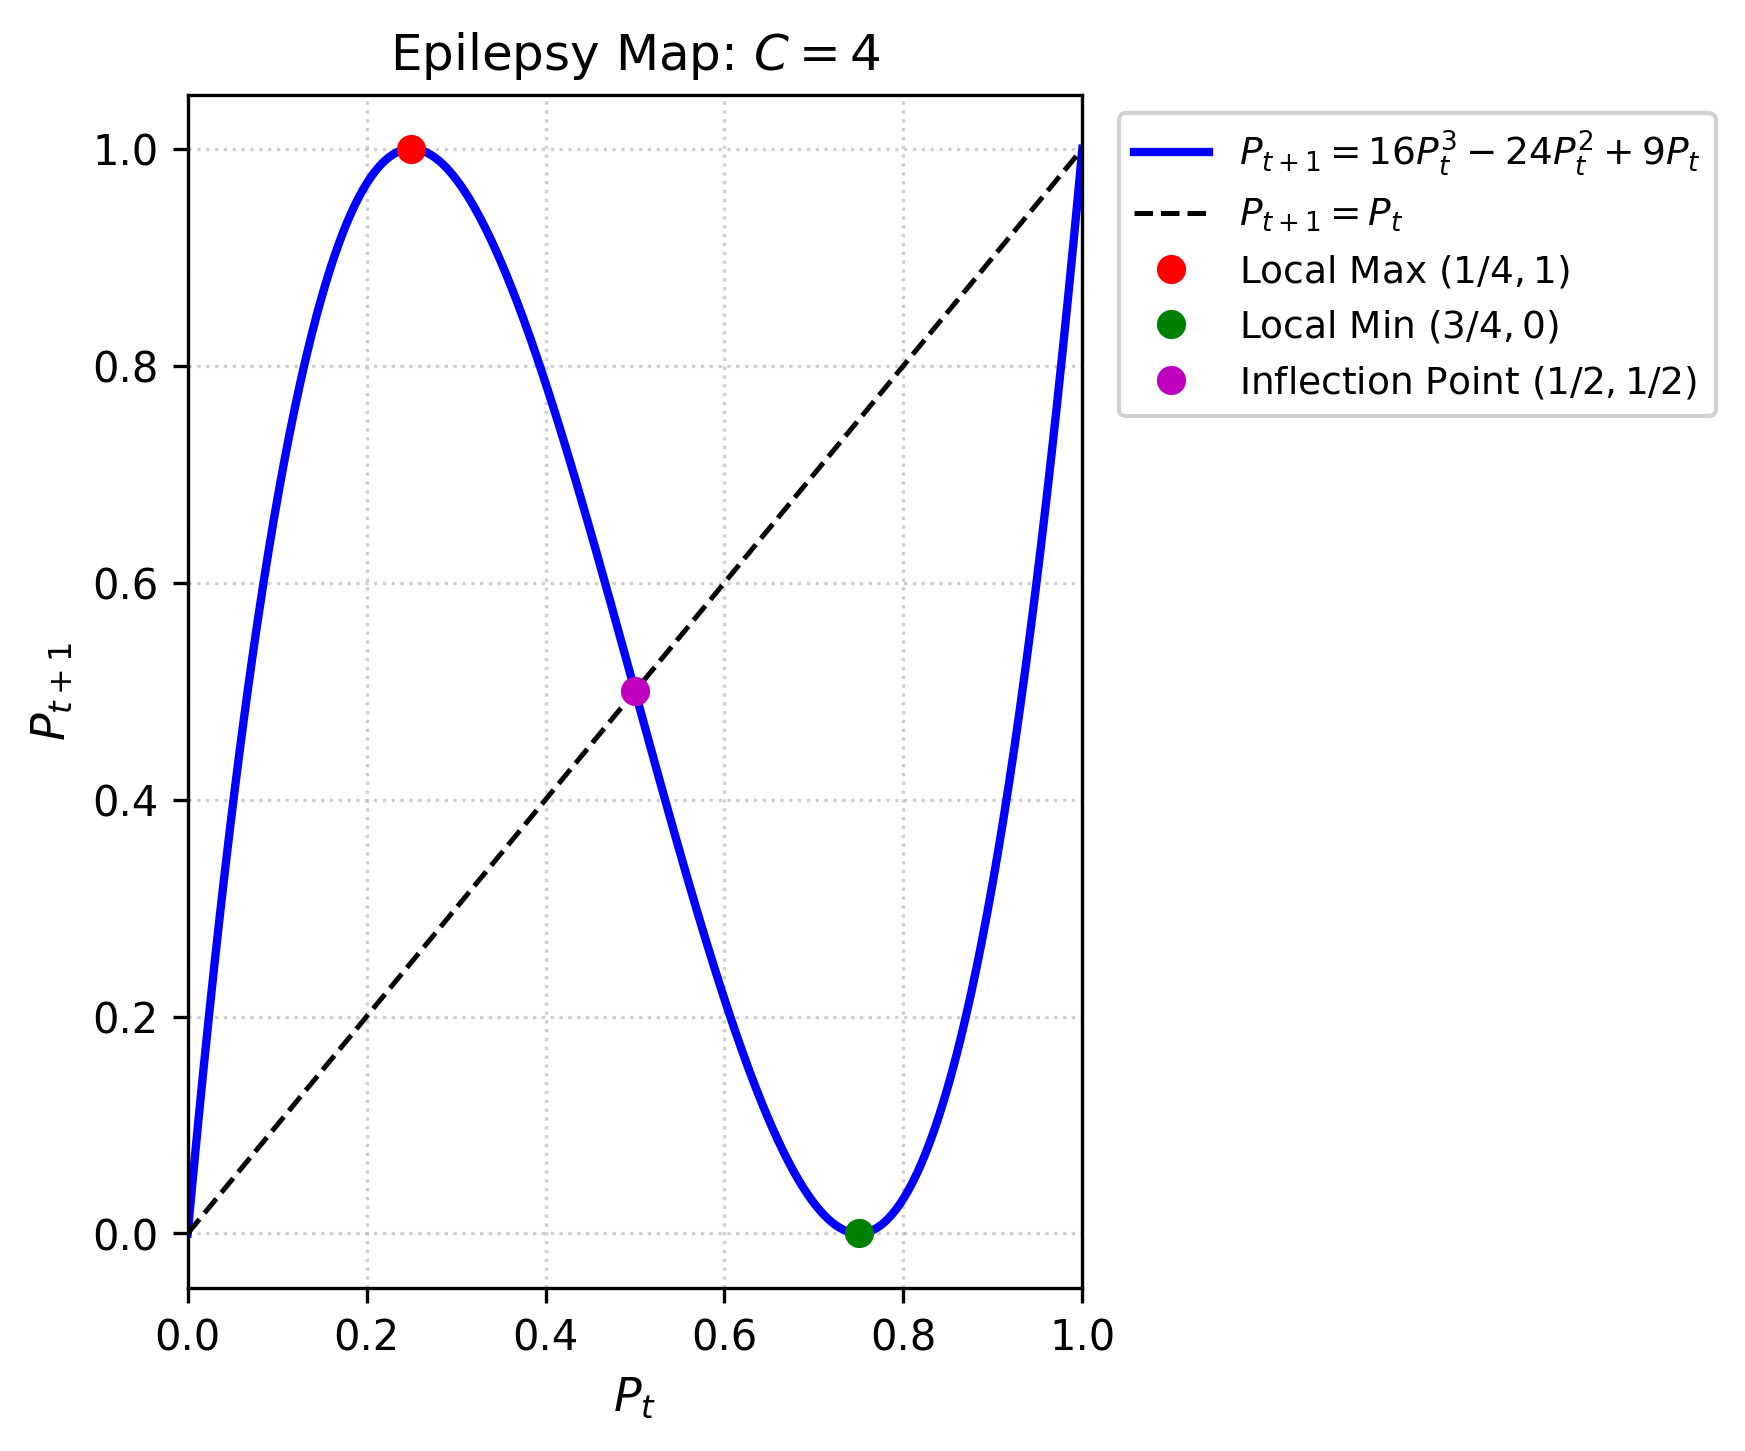
\includegraphics[width=0.6\textwidth]{Epilepsy_Map_C4.png}
    \end{center}
    \item [(d)] Tracing the cobweb diagram starting from $P_0 = 0.45$ with $C = 4$, the iterates don't converge to a fixed point since all three fixed points are unstable ($C = 4 > 2$). Instead, the iterates exhibits chaotic behavior, oscillating between values without settling down to a stable point.
    \begin{center}
    \includegraphics[width=0.6\textwidth]{P4_cobweb.png}
    \includegraphics[width=0.6\textwidth]{P4_time_series.png}
    \end{center}
\end{enumerate}

\subsection*{Problem 5}
Print your last name. Count the number of letters and multiply the number by $0.1$. Your magic number, $m$, is $1$ plus the number that you just computed. If your last name has nine or more letters, assume that $m = 1.9$.\\\\
Consider the finite-difference equation given by the following equations:
\begin{eqnarray*}
x_{t+1} &= m x_t, & 0 \le x_t \le \frac{1}{m} \\
x_{t+1} &= m x_t - 1, & \frac{1}{m} < x_t \le 1
\end{eqnarray*}

\begin{enumerate}
    \item[(a)] Draw a graph of $x_{t+1}$ as a function of $x_t$.
    \item[(b)] Determine the fixed point(s) and determine their stability.
    \item[(c)] Graphically iterate this equation.
    \item[(d)] Are the dynamics chaotic?
\end{enumerate}

\paragraph{Solution} Defining $m$ with last name "Song" (4 letters) gives $m = 1 + 0.4 = 1.4$. 
\begin{enumerate}
    \item [(a)] The graph of $x_{t+1}$ as a function of $x_t$ is shown below:
    \begin{center}
    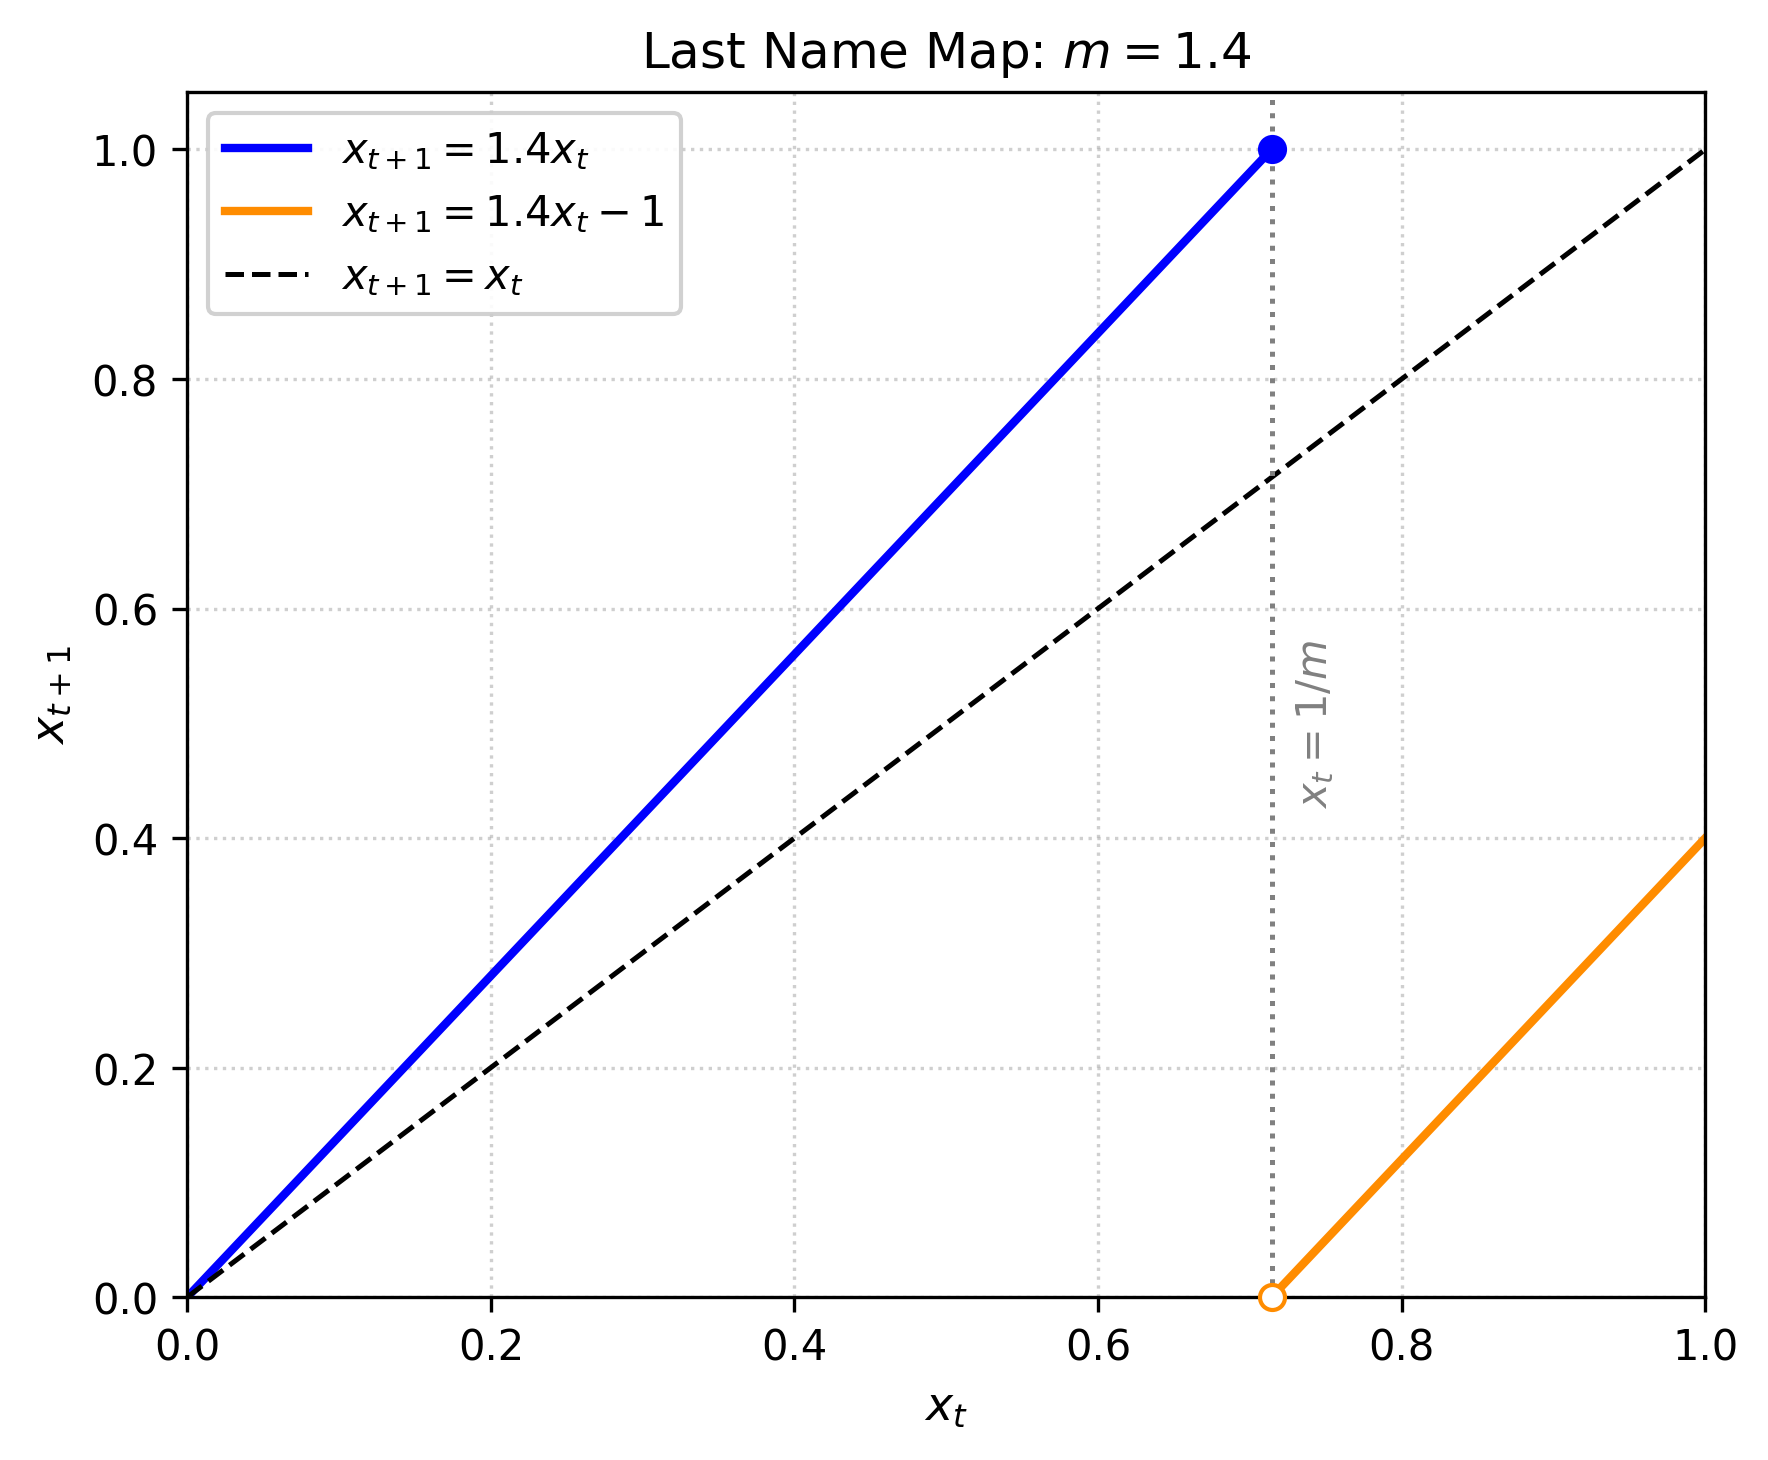
\includegraphics[width=0.6\textwidth]{Problem_5_Map.png}
    \end{center}
    \item [(b)] Fixed points satisfy $x^* = m x^*$ for $0 \le x^* \le 1/m$ and $x^* = m x^* - 1$ for $1/m < x^* \le 1$. Solving these gives:
    \begin{itemize}
        \item For $0 \le x^* \le 1/m$: 
        \[x^* = m x^* \implies x^* (1 - m) = 0 \implies x^* = 0\]
        \item For $1/m < x^* \le 1$:
        \[x^* = m x^* - 1 \implies x^* (1 - m) = -1 \implies x^* = \frac{1}{m - 1}\]
        \[x^* = \frac{1}{1.4 - 1} = 2.5\]
        This is outside the interval $[1/m, 1]$, so there are no fixed points in this range.
    \end{itemize}
    For the only fixed point $x^* = 0$, the stability is determined by the derivative of the map within the interval $[0, 1/m]$:
    \[f'(x) = m \implies f'(0) = 1.4 > 1\]
    Therefore, the fixed point $x^* = 0$ is unstable.
    \item [(c)] Graphical iteration using cobweb diagrams below:
    \begin{center}
    \includegraphics[width=\textwidth]{P5 cobweb.png}
    \includegraphics[width=\textwidth]{P5 time series.png}
    \end{center}
    \item [(d)] The dynamics are chaotic. The iterates do not converge to a fixed point or periodic orbit, instead it oscillates and wraps around itself multiple times in no orderly pattern.
\end{enumerate}



\subsection*{Problem 6}
Show that if there is one solution to $x_m = f(f(x_m))$ where $x_m \ne f(x_m)$ then there must be another, different solution.

\paragraph{Solution} This is a 2-cycle characteristic of a second iterative map. Let $y = f(x_m)$. Then, we have:
\[f(f(y)) = f(f(f(x_m)))\]
Since its given that $x_m = f(f(x_m))$ and $x_m \ne f(x_m)$, thus
\[f(f(y)) = f(f(f(x_m))) = f(x_m) = y \implies f(f(y)) =y\]
Since $y \ne x_m$, we have found another solution.


\subsection*{Problem 7}
Derive and plot the ``3rd iterate'' of the logistic map. Look at problem 10.4.10\footnote{2nd edition problem number} (The birth of period 3) in Strogatz if you like, but beware it could be the beginning of a course project!

\paragraph{Solution} The logistic map is given by the equation:
\[x_{n+1} = r x_n (1 - x_n)\]
Letting $f(x) = r x (1 - x)$, the 2nd iterate is given by:
\begin{eqnarray*}
f(f(x)) &=& r (r x (1 - x)) (1 - r x (1 - x))\\
&=& r^2 x (1 - x) (1 - r x + r x^2)\\
&=& (r^2x-r^2x^2)(1-rx+rx^2)\\
&=& -r^3x^4+2r^3x^3-r^3x^2-r^2x^2+r^2x
\end{eqnarray*}
The 3rd iterate is given by:
\[f(f(f(x))) = r\big[-r^3x^4+2r^3x^3-r^3x^2-r^2x^2+r^2x\big](1-\big[-r^3x^4+2r^3x^3-r^3x^2-r^2x^2+r^2x\big])\]
Plotting the third iterate for varying values of $r$ gives the following:
\begin{center}
    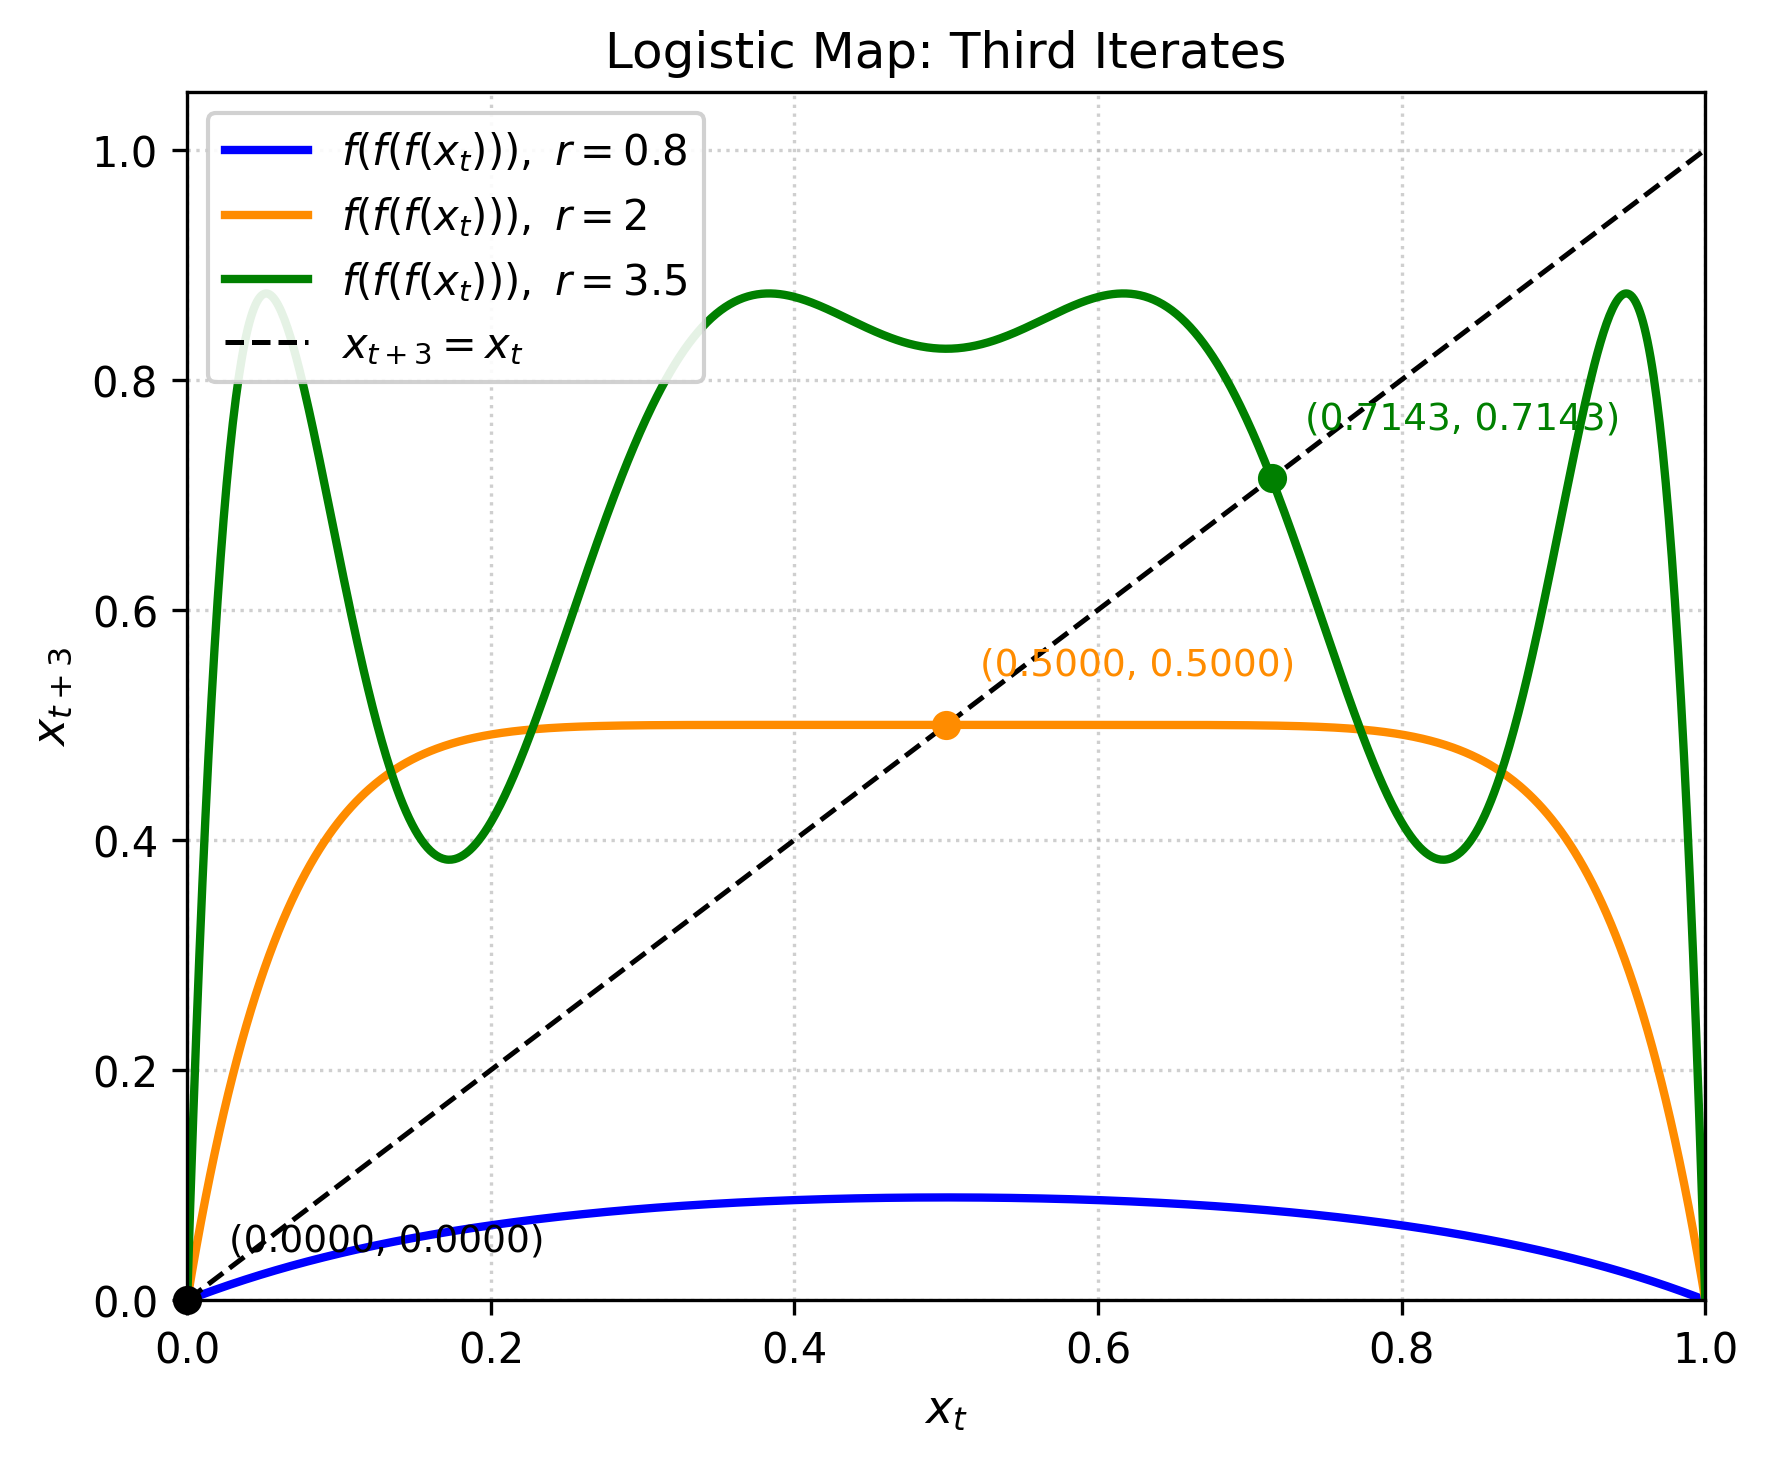
\includegraphics[width=0.6\textwidth]{Logistic Map Third Iterates.png}
    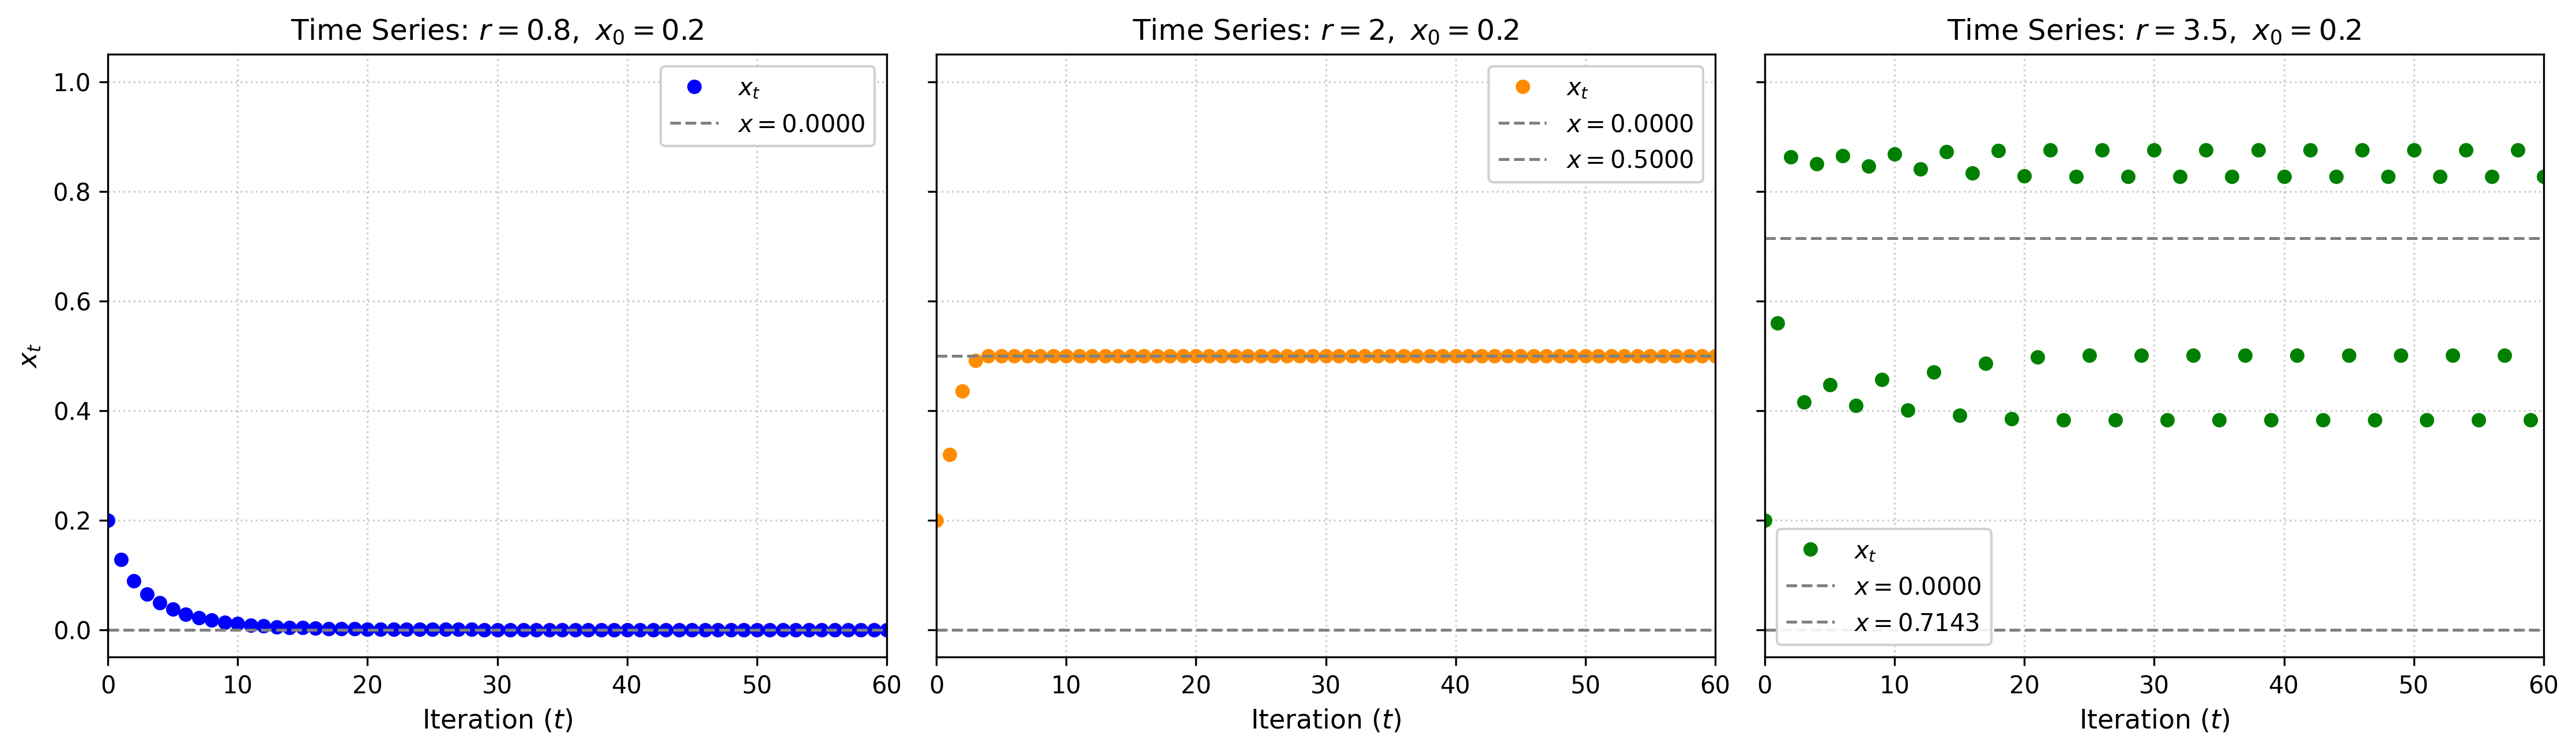
\includegraphics[width=\textwidth]{Logistic Map Time Series.png}
\end{center}


\end{document}